% !TEX encoding = UTF-8
% !TEX TS-program = pdflatex
% !TEX root = ../tesi.tex
% !TEX spellcheck = it-IT

%**************************************************************
\chapter{Conclusioni}
\label{cap:conclusioni}
%**************************************************************

In questo capitolo verranno presentate le riflessioni scaturite dall'analisi effettuata a posteriori dell'esperienza di stage. Verranno analizzati gli obbiettivi raggiunti e l'esperienza acquisita durante il lavoro, concludendo con una valutazione di come la preparazione accademica si interfacci con il mondo del lavoro.

%**************************************************************
\section{Raggiungimento degli obbiettivi}

Lo studente ha raggiunto tutti gli obbiettivi pianificati ad inizio stage, con soddisfazione dell'azienda e del tutor esterno. Questa ha infatti proposto allo studente altri sei mesi di collaborazione per continuare il percorso iniziato e la formazione on-the-job.\\

I tool sviluppati durante la prima parte dello stage sono infatti stati apprezzati e verranno presto inseriti nel modus operandi aziendale. In essi lo studente ha soddisfatto tutti i requisiti posti in fase di analisi degli stessi, seppur sforando di 4 giorni lavorativi sul tempo pianificato per la conclusione definitiva di XML Editor. Tempo recuperato poi durante lo svolgimento della seconda parte.\\

Di seguito viene riportata una tabella ed un grafico contenenti il resoconto della suddivisione delle ore per macro attività ed il confronto fra le ore preventivate e quelle a consuntivo. Le ore riportate di seguito sono comprensive del tempo dedicato alla stesura della documentazione.

\begin{center}
	\begin{longtable}{p{3.2cm}!{\color{white}\vrule width 0.5mm}c!{\color{white}\vrule width 0.5mm}c!{\color{white}\vrule width 0.5mm}c!{\color{white}\vrule width 0.5mm}}
		\rowcolor{headcolor}\textcolor{white}{\textbf{Attività}}&\textcolor{white}{\textbf{Ore a preventivo}}&\textcolor{white}{\textbf{Ore a consuntivo}} & \textcolor{white}{\textbf{Variazione}} \\
		
		\rowcolor{row1} Analisi & 130 & 110 & -20\\
		\rowcolor{row2} Progettazione & 45 & 65 & +20\\
		\rowcolor{row1} Codifica & 85 & 90 & +5\\
		\rowcolor{row2} Verifica & 60 & 55 & -5\\
		\rowcolor{row1} \textbf{Totale} & \textbf{320} & \textbf{320} & \textbf{0}\\
		\caption{Riepilogo ore a preventivo e consuntivo}
		\label{tab:istoBilancio}
	\end{longtable}
\end{center}

\begin{figure}[h!] 
	\centering 
	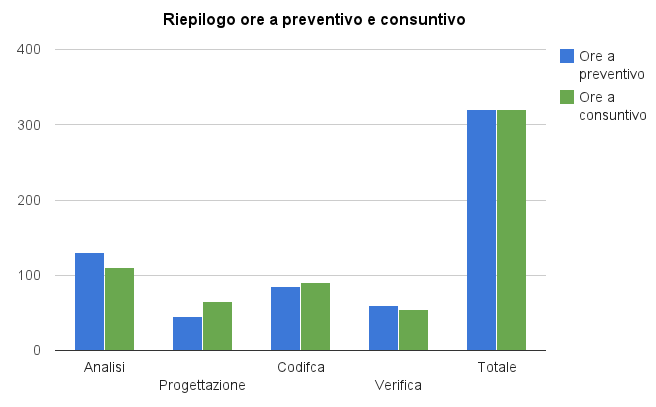
\includegraphics[width=1\columnwidth]{bilancio.png} 
	\caption{Istogramma del riepilogo ore a preventivo e consuntivo}
	\label{fig:istoBilancio}
\end{figure}

\newpage

Come visibile in tabella \ref{tab:istoBilancio} ed in figura \ref{fig:istoBilancio} si nota che l'attività di analisi e formazione ha occupato 20 ore meno del previsto, le quali sono state quasi tutte reinvestite in progettazione, spiegabile dalla complessità del sistema con il quale lo studente ha interagito.\\

La codifica invece ha portato via poco in più di ciò preventivato e, vista l'impossibilità di aumentare il budget ore complessivo, si è stati costretti a tagliare sulla verifica.

%**************************************************************
\section{Conoscenze acquisite e valutazione della preparazione accademica}

Lo studente ha approfondito la sua conoscenza delle librerie Qt\textsuperscript{\textregistered}, soprattutto ha potuto maturare esperienza nella progettazione di un'architettura che si adattasse al meglio con il framework in questione e che al contempo risultasse facilmente comprensibile ed estendibile. Egli ha potuto inoltre mettere in pratica le conoscenze di usabilità nel progettare la user interface dei tool, acquisite nei corsi di Tecnologie Web.\\

Lo stagista ha inoltre potuto approfondire le proprie conoscenze nella grafica 3D, sopratutto nell'ambito delle animazioni scheletrali. C'è da dire, sotto questo aspetto, che le competenze necessarie per svolgere gli obbiettivi della seconda parte sono state acquisite dallo studente in maniera autonoma durante tutto il percorso di studi, utilizzando come basi per comprendere le nuove nozioni ciò studiato durante il percorso accademico.\\

Tranne le conoscenze di grafica 3D bisogna affermare che la preparazione fornita durante il percorso di studi è stata adeguata alle necessità aziendali. Durante lo sviluppo si è potuto constatare che il metodo di lavoro acquisito si adattava bene a quello aziendale.\\

Si è constatato inoltre la necessità di autonomia nella ricerca e nell'approfondimento di particolare tematiche di cui lo studente non era a conoscenza con gli strumenti a disposizione (internet e manuali).\\

Tutto il codice prodotto, sopratutto quello dei tool, è stato documentato nel migliore dei modi per poter permettere a chiunque di comprenderlo ed evolverlo in completa autonomia.\\

È convinzione dello studente che, al di là degli aspetti teorici e pratici di qualunque tecnologia, un informatico maturo che abbia compreso gli aspetti fondamentali dell'informatica insegnati in questo corso di studio, potrà durante la sua intera carriera acquisire senza troppi problemi tutte le tecnologie di cui avrà bisogno.

%**************************************************************
\section{Valutazione personale}

Lo studente ritiene che lo stage sia stata un'esperienza decisamente positiva, oltre agli obbiettivi raggiunti, l'ambiente in cui è stato inserito si è dimostrato positivo e amichevole. La positività che lo stagista ha sempre dimostrato è stata ricambiata dai colleghi e dalla direzione che ha confermato la collaborazione. Altro motivo di crescita è derivato dal trasferimento a Milano, sede di Milestone S.r.l., per lo svolgimento del tirocinio, che ha permesso allo studente di crescere e maturare anche da questo punto di vista.\\

Per tutti questi motivi si afferma la buona riuscita del periodo di stage.
